\chapter{Lektion 1}
\section{Kapitel 1}
\subsection{Economics: studying choice in a world of scarcity(mangel)}
\textbf{Økonomi} er studiet om hvordan folk vælger at bruge penge når der er mangler og resultaterne af disse valg. Fx. En klasse med 100 er billigere end en med 20, men det svækker også kvaliteten. 
\begin{defn}\textbf{The Scarcity Principle} %Ny definition
\newline
Der er altid flere behov end ressourcer. Dette betyder at have mere af en ting fører til mindre af en anden. 
\end{defn}
\begin{defn}\textbf{The Cost-Benefit Principle} %Ny definition
\newline
Man burde kun handle hvis fordelene overskrider bekostningen.
\end{defn}
Det er selvfølgelig forskelligt hvad man mener er værd at bruge på forskellige ting. 

\subsection{Applying the Cost-Benefit Principle}
Man er \textbf{rationel} hvis man har vel definerede mål og prøver at opnå dem bedst muligt. CBP bruges til at studere rationelle menneskers valg. Nabo sælger spil og føtex sælger spil. Føtex sælger det til 10 kr mindre end Nabo, er turen til Føtex mere eller mindre værd end 10kr?(Cost-Benefit Principle) Hvis du synes turen til Føtex koster 9 kr er der \textbf{økonomisk overskud}. \textbf{Offeromkostningerne} er det du skal opgive(ofre) for at gøre noget, fx hvis du går i Føtex kan du ikke nå at se den film du gerne vil se. 

CBP kan hjælpe med at træffe bedre beslutninger. Og den kan bruges til at forudse folks beslutninger. 

\subsection{Three important decision pitfalls}
\textbf{Pitfall 1:}\\
Det er svært at måle fordele og ulemper ved handlinger ift penge. \\
\textbf{Pitfall 2:}\\
Man overser de implicitte ting(ikke tydelige). Hvis man bruger en rabat kupon på noget ikke nødvendigt fordi det kan betale sig og derfor ikke bruger den på noget man SKAL, er det ikke længere sikkert at det kan betale sig. \\
\textbf{Pitfall 3:}\\
Ulemper er de ting man kun kan undgå ved ikke er gøre en ting og fordele er de ting der kun kan ske hvis vi gøre det. \textbf{Sunkne omkostninger} er de ting man ikke kan lave om på beslutning(ikke refunderbare flybilletter)\\
\textbf{Marginal omkostningerne} er stigningen i omkostningerne som resultat af en "aktivitet". \textbf{Marginal fordel} er stigningen i fordelene som resultat af en "aktivitet". Så længe marginal fordelene overstiger marginal omkostningerne kan antallet af "aktiviter" hæves. Her er det ikke nok bare at se på gennemsnitlig fordele og ulemper, da det man ikke ved hvad en ekstra aktivitet gør. 

\subsection{Normative economics versus positive economics}
CBP er en et 
\textbf{normativt økonomisk princip}, hvilket betyder guide til hvordan man \textit{burde} vælge. CBP er dog ikke altid et \textbf{
positivt økonomisk princip} der betyder guide til hvordan man \textit{vil} handle. 
\begin{defn}\textbf{The incentive principle} %Ny definition
\newline
Man er mere villig til at lave en aktivitet hvis fordelen stiger og mindre villig hvis ulempen stiger. Dette er et positivt økonomisk princip
\end{defn}

\subsection{Economics: micro and macro}
Mikro: person og gruppe\\
Makro: National


\section{Kapitel 3}
\subsection{What, how, and for whom? central planning versusthemarket}
En centraliseret økonomisk organisering er hvor man selv laver det man skal bruge, fx i gamle dage sørgede hver klan for at producere det mad de spiste og en leder tog alle "økonomiske" beslutninger. Dette er ikke særlig udbredt i dag og ses næsten kun små selvforsynende samfund og lidt i kommunistiske samfund fx cuba. 

På den anden side er der det \textbf{frie marked}. Der  er ikke noget rigtigt fri marked, men det er det man kalder det. Det er en mere effektiv form, da produktion og forbrug bestemmes af hver enkelte. 

\subsection{Buyers and sellers in markets}
\textbf{Markedet} for enhver varer består af alle sælgere og købere af varen. Efter mange år med tvivl er man kommet frem til at \textbf{markedsprisen} på en varer afhænger ikke bare om villighed mm, men af udbud og efterspørgsel. 

\subsubsection{The demand curve} 
\textbf{Efterspørgsleskurven} er en relation mellem mængden af en varer folk vil købe i forhold til prisen. Hældningen er negativ da når prisen falder, stiger efterspørgslen. \textbf{Substitutions effekten} er det der sker hvis prisen på pizza stiger og som resultat køber folk istedet en burger. \textbf{Indkomst effekten} er når prisen stiger og folk ikke har råd til at købe lige så mange stykker pizzaer og dermed falder efterspørgslen af pizza. \textbf{Køberens reservationspris} er den maksimale pris de vil give for en varer. Det skal dog påpeges at folk ikke har samme reservationspris. 

\subsubsection{The supply curve}
\textbf{Udbudskurven}  foræller om hvor meget sælgere er villig til at sælge deres vare for. Dette afhænger af om en sælger kan tjene mere for en varer end at investere pengene i noget andet, \textbf{offeromkostningerne}. Derfor har udbudskurven også en positiv hældning. \textbf{Sælgers reservationspris} for at sælge en enhed mere er marginal omkostningerne for at producere den. 

\subsection{Market equilibrium}
Der er \textbf{ligevægt} i et system når resultatet er i balance eller ved en situation der ikke ændres. Hvis man vil bestemme \textbf{ligevægts prisen} og \textbf{enhedsligevægten} skal man bestemme \textbf{markedsligevægten}. I vores system er det der hvor efterspørgsel- og udbudskurverne skærer hinanden. Det er her hvor både sælger og køber er "tilfredse". Hvis prisen er over ligevægtsprisen er der overskydende udbud og omvendt for efterspørgsel. Naturligt vil markedet bevæge sig mod ligevægt.

Regering, love mm kan sætte et \textbf{prisloft}, fx kan det være forbudt at tage mere end 60kr for en pizza. 

\subsection{Predicting and explaining changes in prices and quantities}
Hvis der er en \textbf{ændring i mængden af efterspørgsel} bevæger man sig langs kurven, og hvis der er en \textbf{ændring i efterspørgsel} forskydes kurven. På samme måde følger udbuddet. 

Hvis to ting er \textbf{komplimentære}. Vil en stigning af den ene fører til et fald af den anden.

Hvis to ting er \textbf{erstatninger}, vil et fald for den ene føre til et fald i den anden.

En \textbf{normal vare} er en vare hvis efterspørgselskurve forskydes mod højre hvis køberes indkomst stiger og til venstre hvis den falder. 

En \textbf{ringere vare} er en vare hvis efterspørgselskurve forskydes mod venstre hvis køberes indkomst stiger og til højre hvis den falder. Dette er varer som kan erstattes af fx noget mere sikkert. 

\begin{eks} \textbf{} %Nyt eksempel
\newline
Hvis det pludselig koster mindre at spille tennis på en tennisbane, vil folk spille mere tennis og der er mere brug for tennisbolde. Her vil der være en ændring i efterspørgsel, så kurven flyttes mod højre. Hvis der er to former for tennisbolde, 1 og 2. Vil et fald i prisen på 1, gøre at efterspørgslen på 2 falder og der vil ske en ændring i efterspørgsel. Dermed vil kurven flyttes mod højre. Derimod vil der ske en ændring i mængden af efterspørgsel for 1. 
\end{eks}

\subsubsection{Shift in the supply curve}
\begin{eks} \textbf{} %Nyt eksempel
\newline
Skateboard laves bla. af fiberglas. Hvis prisen for fiberglas stiger vil marginal omkostningerne for at producere et skateboard stige og der er dermed færre hvor prisen kan dække offeomkostningerne og udbuddet falder. Altså forskydes udbudskurven mod venstre. 
\end{eks}

For det meste gør teknologisk fremgang også at udbudskurven forskydes mod højre da det bliver nemmere og billigere at producere ting. 

\subsubsection{Four simple rules}
\includegraphics[scale=0.8]{Afsnit/Lektion1/Udbudefterspørgsel.png}

\subsection{Efficiency and equilibrium}
\subsubsection{Cash on the table}
\textbf{Købernes overskud} er forskellen mellem deres reservationspris og den egentlige pris. \textbf{Sælgernes overskud} er forskellen mellem den modtaget pris og sælgerens reservationspris. \textbf{Total overskud} er forskellen mellem sælgers- og købers reservationspris eller summen af de to overskud. 

Når de fælles fordele ikke er opnået, altså at markedet ikke er i ligevægt, kalder økonomer det "cash on the table". 

\subsubsection{Smart for one, dumb for all}
\textbf{Social optimal mængde} for enhver varer er mængden der maksimere det totale økonomiske overskud. Det er der hvor marginal omkostningerne og marginal fordele er de samme. \textbf{Effektivitet} er når alle varer og services er "brugt" til deres socialt optimale niveau. 

\begin{defn}\textbf{The efficiency principle} %Ny definition
\newline Det er et vigtigt socialt mål fordi når hele økonomien stiger, vil alle i økonomien nyde godt af det. 
\end{defn}

\begin{defn}\textbf{The equilibrium principle} %Ny definition
\newline 
Et marked i ligevægt er der ingen uudnyttede muligheder for enkeltpersoner, men udnytter muligvis ikke alle gevinster, der er opnåelige gennem kollektiv handling
\end{defn}

\section{Kapitel 4}
\subsection{Price elasticity of demand} 
For nogle varer som foreksempel salt, vil en fordobling i pris ikke nødvendigvis betyde at folk ændre deres salt vaner og køber mindre, men for andre ting som en yacht ville mange lade være med at købe en hvis prisen fordobles. 
\subsubsection{Price elasticity defined}
\begin{defn}\textbf{Priselastisiteten for efterspørgsel} %Ny definition
\newline
Priselastisiteten for efterspørgsel af en varer en et mål for reaktionsevnen for mængden af varen ud fra en prisændring. Ændringen i mængden ved en 1\% ændring i prisen. 
\end{defn}
Prisen falder med 1\%, mængden stiger med 2\%. Så er elastisiteten -2\%. Det kan også beregnes ved 
\begin{align*}
    \frac{\text{Procentvis ændring i mængden}}{\text{Procentvis ændring i prisen}} = \frac{2}{-1}=-2
\end{align*}
Den vil for efterspørgsel altid være negativ da pris og mængde altid bevæger sig i hver sin retning afhængig af hinanden. Efterspørgslen er \textbf{elastisk} hvis |elastisiteten|$>1$, \textbf{uelastisk} hvis |elastisiteten|$<1$ og \textbf{enheds elastisk} hvis |elastisiteten|$=1$.

\subsubsection{Determinants of price elasticity of demand}
Der er flere ting der kan afgøre priselastisiteten af en varer. Hvad skal der til for at man ved en prisstigning ikke længere vil have varen?

\textbf{Substitutions muligheder}
Elastisiteten stiger hvis det er en varer hvor der findes et produkt der næsten kan gøre det samme. Hvis prisen stiger på den ene varer vil man man kunne skifte til den anden. 

\textbf{Budgetandel}
Dyrer varer har en tendens til at have højere priselastisitet. Det gør de da de udgør en større andel af ens budget. Hvis en nøglering steg fra 10kr til 20kr, ville mange være ligeglade og stadig købe en nøglering de få gange man skulle det. Hvis en bil derimod fordobles i pris ville man gå ud og lede efter andre billigere modeller. 

\textbf{Tid}
Elasticiteten for efterspørgsel på enhver varer er højere på lang sigt end på kort sigt. 

\subsubsection{Some representative elasticity estimates}
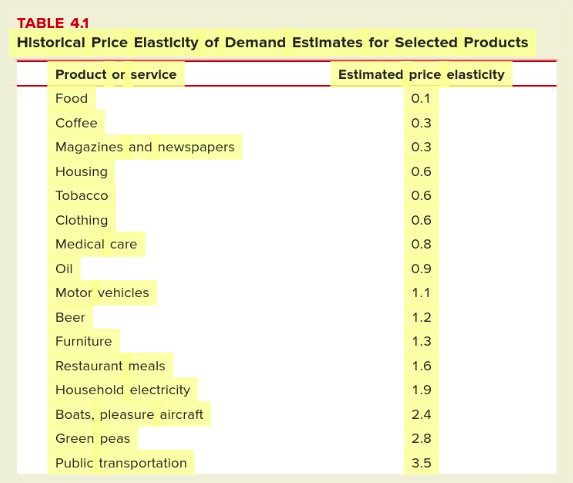
\includegraphics[scale=0.8]{Afsnit/Lektion1/Elastisitet.png}

\subsection{A graphical interpretation of price elasicity}
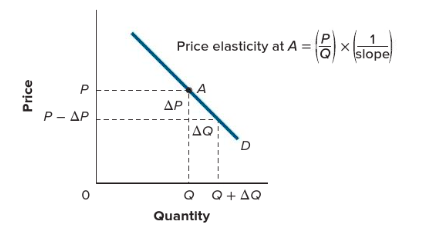
\includegraphics[scale=0.8]{Afsnit/Lektion1/Elastisitetgraf.png}
\begin{align*}
    \text{Priselastisitet} = \in \frac{\frac{\Delta Q}{Q}}{\frac{\Delta P}{P}}
\end{align*}
Hvis man skal bestemme den i et bestemt punkt bruges formlen på grafen. 
\begin{eks} \textbf{} %Nyt eksempel
\newline
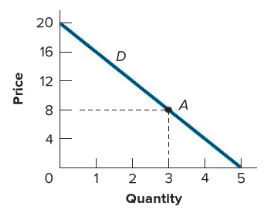
\includegraphics[scale=0.8]{Afsnit/Lektion1/Elastisiteteks.png}

Hvis man skal beregne priselastisiteten i A ser man på forholdet mellem skæring med y og x-aksen.
\begin{align*}
    \frac{1}{\text{slope}} = \frac{1}{\frac{20}{5}}= \frac{1}{4}
\end{align*}
Så ser vi på forholdet mellem mængde og pris i A.
\begin{align*}
    \frac{P}{Q} = \frac{8}{3}
\end{align*}
Dermed har vi
\begin{align*}
    \in_A = \frac{8}{3} \times \frac{1}{4} = \frac{2}{3}
\end{align*}
Det vil sige at når prisen er 8 vil et 3\% fald i pris medfører en stigning på 2\% i mængden
\end{eks}

\subsubsection{Price elasticity changes along a straight-line demand curve}
På midtpunktet af kurven vil priselastistiteten altid være 1. Hvis den er under midtpunktet vil den være under 1 og samme med over. 
\subsubsection{Two special cases}
Det ovenstående gælder selvfølgelig ikke at hvis efterspørgselskurven er vandret er hældningen 0 og derfor er priselastisiteten uendelig ved hvert punkt. Dette kaldes \textbf{perfekt elastisk}. Hvis den er lodret er hældningen uendelig og derfor er priselastisiteten 0 ved hvert punkt. Dette kaldes \textbf{perfekt uelastisk}.

\subsection{Elasticity and total expenditure}
Sælgere er interesseret i at vide hvor meget de kan tage for en vare. Hvis man antager det samlede forbrugere bruger på et produkt er sælgers samlede indtægter. Hvis man har at man kan sælge 500 billetter til 2kr og 400 til 4kr. Vil man vælge at sælge til 4kr da indtjeningen er 1000kr ift 1600kr. Hvis man kun kunne sælge 200 billetter hvis man satte dem til 4kr, ville man vælge de 2kr. 

Ved at beregne på denne måde er det muligt at bestemme den optimale prise for sælger. Dette er ved midtpunktet af efterspørgselskurven. 

\textbf{Regl nr. 1}: Hvis priselastisiteten er over 1, vil prisen og samlede indtægt bevæge sig i hver sin retning. 

\textbf{Regl nr. 2}:  Hvis priselastisiteten er under 1, vil prisen og samlede indtægt bevæge sig i samme retning. 

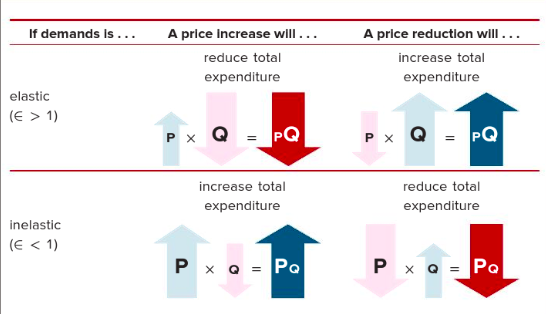
\includegraphics[scale=0.8]{Afsnit/Lektion1/ElastisitetPQ.png}

\subsection{Income elasticity and cross-price elasticity of demand}
\textbf{Krydspriselasticitet af efterspørgsel} er ændring i mængden af en varer ift ændring af pris på en komlementær/erstatning varer. Hvis elasticiteten er negativ er de komplementær vare og hvis den er positiv er de erstatninger. 
\textbf{Indkomstelasticitet af efterspørgsel} er ændring i mængden af en varer ift indkomsten.

\subsection{The price elasticity of supply}
\begin{defn}\textbf{Priselasisiteten for udbud} %Ny definition
\newline
\textbf{Priselasisiteten for udbud} er den procentvise ændring i mængden af udbud ved en prisændring på 1\%
\end{defn}
Den beregnes på samme måde som priselastisiteten for efterspørgsel også i hvert punkt, den er bare altid positiv. Den er altid 1 hvis udbudskurven går gennem origo. Hvis den er lodret er der perfekt uelastisk, vandret perfekt elastisk.

\subsubsection{Determinants of supply elasticity}
Jo nemmere det er at skaffe yderligere input jo højere er priselastisiteten. 
\textbf{Fleksibilitet af inputs}: Hvis et input også kan bruges til et andet produkt kan man tage input derfra og dermed gøre varen relativ elastisk. Det er fx nemt at skaffe folk der kan lave lemonade men svært at skaffe hjerne kiruger. 

\textbf{Mobility of inputs}: Hvis det er nemt at transportere et input, kan man ved en stigning i prisen på et marked gøre det muligt at søge over på et andet marked hvor det måske er billigere. Landbrugsprodukter  er mere elastiske da landmænd er villige til at migrere nord til vækstsæsonen. Priselastisiteten for mange ting stiger hver gang en ny motorvej bliver bygget.

\textbf{Ability to produce substitute inputs}: Hvis der kommer en erstatning vil priselastisiteten stige.

\textbf{Time}: Da det tager tid at skift varer, bygge maskiner mm. Vil elastisiteten være højere på lang sigt end kort sigt.

Flygtige priser er også almindelige i markeder hvor efterspørgselskurverne svinger kraftigt og udbudskurven er meget uelastisk.

\subsubsection{Unique and essential inputs: the ultimate supply bottleneck}
Det er bare ikke altid muligt at få de nødvendige inputs, fx hvis du vil starte et NBA team. De gode spillere er for dyre. På lang sigt er unikke og nødvendige input den sande flaskehals for udbud. 

\subsection{Vigtigt fra forelæsningen}
\textbf{Efterspørgsel}
Efterspørgselskurven laves ud fra reservationspriser. Ved 4kr er der 8000 der vil købe.

Langs kurven, prisen stiger eller falder. 
Kurven flytter sig, prisen på komplementære(ski(pris op), leje til lift(flytter til venstre)) eller substitutter ændres(æble(pris stiger) og appelsinjuice(kurve til højre)). Indkomst stiger, kurve til højre(normal goder). præferencer, befolkningen(fx størrelse) og foventninger(elbil) kan også rykke kurven.

\textbf{Udbud}
Igen er det udbydernes reservationspris der afgør kurven. 

Langs kurven, pris ændres

Kurven flytter, prisen på input ændres(pris på mel stiger, kurve for pizza mod venstre) eller teknologien forbedres(kurve mod højre). Vejret, antal udbydere og forventninger kan også påvirke udbuddet.

\textbf{Ligevægt}
Alle vil gå efter ligevægt.

\textbf{Efterspørgsels priselasticitet}
Hvis kurven skærer y-aksen i a og x-aksen i b, gælder det i ($\frac{b}{2}, \frac{a}{2}$) at $\in = 1$. For på højresiden af $\frac{b}{2}$, $\in<1$ og venstresiden af $\frac{b}{2}$, $\in>1$.

Jo mere stejl en kurve er jo lavere er priselasticiteten. 

\textbf{Monopol}
Når man selv kan vælge en pris vil man aldrig sætte prisen sådan at den er ikke elastisk. Man vil hæve prisen. På samme måde vil man sænke prisen hvis den er elastisk. Man vil gå efter enhedselasticitet da det er den optimale omsætning. 

\textbf{Øvrige elasticiteter}

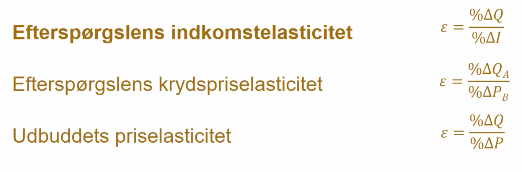
\includegraphics[scale=0.8]{Afsnit/Lektion1/andre.png}


















